\section{Estimating Constant Speciation \& Extinction Rates}

\subsection{Outline}

This tutorial describes how to specify basic branching-process models in \RevBayes;
two variants of the constant-rate birth-death process \citep{Yule1925,Kendall1948,Thompson1975,Nee1994b,Rannala1996,Yang1997,Hoehna2015a}.
The probabilistic graphical model is given for each component of this tutorial.
After each model is specified, you will estimate speciation and extinction rates using Markov chain Monte Carlo (MCMC).
Finally, you will estimate the marginal likelihood of the model and evaluate the relative support using Bayes factors.

\subsection{Requirements}
We assume that you have read and hopefully completed the following tutorials:
\begin{itemize}
\item RB\_Getting\_Started
\item RB\_Basics\_Tutorial
\item RB\_BayesFactor\_Tutorial
\end{itemize}
Note that the RB\_Basics\_Tutorial introduces the basic syntax of \Rev but does not cover any phylogenetic models.
You may skip the RB\_Basics\_Tutorial if you have some familiarity with \R.
The RB\_BayesFactor\_Tutorial introduced Bayesian model selection by means of Bayes factors, which can be skipped by readers familiar with Bayesian model selection.
We tried to keep this tutorial very basic and introduce all the language concepts and theory on the way.
You may only need the RB\_Basics\_Tutorial for a more in-depth discussion of concepts in \Rev.


%%%%%%%%
%%   Data   %%
%%%%%%%%
\section{Data and files}

We provide the data file(s) which we will use in this tutorial.
You may want to use your own data instead.
In the \cl{data} folder, you will find the following files
\begin{itemize}
\item \cl{primates\_springer.tre}: Dated primates phylogeny including 369 species from \cite{Springer2012}.
\end{itemize}


\impmark{Open the tree \cl{data/primates\_springer.tre} in FigTree. }


\bigskip
\section{Pure-Birth (Yule) Model}\label{yuleModSec}

Before evaluating the relative support for different models, we must first specify them in \Rev.
In this section, we will walk through specifying a pure-birth process model and estimating the marginal likelihood. 
The section about the birth-death process will be less detailed because it will build up on this section.

The simplest branching model is the \emph{pure-birth process} described by \cite{Yule1925}. 
Under this model, we assume at any instant in time, every lineage has the same speciation rate $\lambda$.
In its simplest form, the speciation rate remains constant over time. 
As a result, the waiting time between speciation events is exponential, where the rate of the exponential distribution is the product of the number of extant lineages ($n$) at that time and the speciation rate: $n\lambda$ \citep{Yule1925,Aldous2001,Hoehna2014a}. 
The pure-birth branching model does not allow for lineage extinction (\IE the extinction rate $\mu=0$). 
However, the model depends on a second parameter $\rho$ which is the probability of sampling a species in the present time as well as the time of the start of the process, whether that is the origin time or root age.
Therefore, the probabilistic graphical model of the pure-birth process is quite simple, where the observed time tree topology and node ages are conditional on the speciation rate, sampling probability, and root age (Fig.~\ref{yuleGMfig}).
\begin{figure}[h!]
\centering
\fbox{\includegraphics[width=3in]{\ResourcePath figures/yule_gm.eps}}
\caption{\small The graphical model representation of the pure-birth (Yule) process.}
\label{yuleGMfig}
\end{figure}

We can add hierarchical structure to this model and account for uncertainty in the value of the speciation rate by placing a hyperprior on $\lambda$ (Fig.~\ref{yuleGMfig2}). 
The graphical models in Figures \ref{yuleGMfig} and \ref{yuleGMfig2} demonstrate the simplicity of the Yule model. 
Ultimately, the pure birth model is just a special case of the birth-death process, where the extinction rate (typically denoted $\mu$) is a constant node with the value 0. 
\begin{figure}[h!]
\centering
\fbox{\includegraphics[width=4in]{\ResourcePath figures/yule_gm2.eps}}
\caption{\small The graphical model representation of the pure-birth (Yule) process, where the speciation rate is treated as a random variable drawn from a lognormal distribution.}
\label{yuleGMfig2}
\end{figure}

For this exercise, we will specify a Yule model, such that the speciation rate is a stochastic node, drawn from a lognormal distribution as in Figure \ref{yuleGMfig2}.
In a Bayesian framework, we are interested in estimating the posterior probability of $\lambda$ given that we observe a time tree.
\begin{align}\label{bayesTher}
\mathbb{P}(\lambda \mid \Psi) &= \frac{\mathbb{P}(\Psi \mid \lambda)\mathbb{P}(\lambda \mid \nu)}{\mathbb{P}(\Psi)}
\end{align}
In this example, we have a phylogeny of all living primates. 
We are treating the time tree $\Psi$ as an observation, thus clamping the model with an observed value.
The time tree we are conditioning the process on is taken from the analysis by \citet{Springer2012}.
Furthermore, there are approximately 450 described primates species, so we will fix the parameter $\rho$ to $369/450$.


\exs{The full Yule-model specification is in the file called \href{https://github.com/revbayes/revbayes_tutorial/raw/master/RB_DiversificationRate_Tutorial/RevBayes_scripts/Yule.Rev}{\cl{Yule.Rev}} on the \RevBayes tutorial repository.}

\subsection{Read the tree}

Begin by reading in the observed tree. 

{\tt \begin{snugshade*}
\begin{lstlisting}
T <- readTrees("data/primates_springer.tre")[1]
\end{lstlisting}
\end{snugshade*}}

From this tree, we can get some helpful variables:
{\tt \begin{snugshade*}
\begin{lstlisting}
taxa <- T.taxa()
\end{lstlisting}
\end{snugshade*}}

Additionally, we can initialize an iterator variable for our vector of moves:
{\tt \begin{snugshade*}
\begin{lstlisting}
mvi = 0
mni = 0
\end{lstlisting}
\end{snugshade*}}


\subsection{Specifying the model}

\subsubsection{Birth rate}

The model we are specifying only has three nodes (Fig.~\ref{yuleGMfig2}). 
We can specify the birth rate $\lambda$, the mean and standard deviation of the lognormal hyperprior on $\lambda$, and the conditional dependency of the two parameters all in one line of \Rev code.
{\tt \begin{snugshade*}
\begin{lstlisting}
birth_rate_mean <- ln( ln(450/2) / T.rootAge() )
birth_rate_sd <- 0.587405
birth_rate ~ dnLognormal(mean=birth_rate_mean,sd=birth_rate_sd) 
\end{lstlisting}
\end{snugshade*}}
Here, the stochastic node called \cl{birth\_rate} represents the speciation rate $\lambda$.
\cl{birth\_rate\_mean} and \cl{birth\_rate\_sd} are the prior mean and prior standard deviation, respectively.
We chose the prior mean so that it is centered around observed number of species (\IE the expected number of species under a Yule process will thus be equal to the observed number of species) and a prior standard deviation of 0.587405 which creates a lognormal distribution with 95\% prior probability spanning exactly one magnitude.
If you want to represent more prior uncertainty by, \EG allowing for two orders of magnitude in the 95\% prior probability then you can simply multiply \cl{birth\_rate\_sd} by a factor of 2.

To estimate the value of $\lambda$, we assign a proposal mechanism to operate on this node. 
In \RevBayes these MCMC sampling algorithms are called \emph{moves}. 
We need to create a vector of moves and we can do this by using vector indexing and our pre-initialized iterator \cl{mi}.
We will use a scaling move on $\lambda$ called \cl{mvScale}.
{\tt \begin{snugshade*}
\begin{lstlisting}
moves[++mvi] = mvScale(birth_rate,lambda=1,tune=true,weight=3)
\end{lstlisting}
\end{snugshade*}}

\subsubsection{Sampling probability}

Our prior belief is that we have sampled 367 out of 450 living primate species. 
To account for this we can set the sampling parameter as a constant node with a value of 369/450
{\tt \begin{snugshade*}
\begin{lstlisting}
rho <- T.ntips()/450
\end{lstlisting}
\end{snugshade*}}


\subsubsection{Root age}

Any stochastic branching process must be conditioned on a time that represents the start of the process. 
Typically, this parameter is the \textit{origin time} and it is assumed that the process started with \textit{one} lineage. 
Thus, the origin of a birth-death process is the node that is \textit{ancestral} to the root node of the tree.
For macroevolutionary data, particularly without any sampled fossils, it is difficult to use the origin time.
To accommodate this, we can condition on the age of the root by assuming the process started with \textit{two} lineages that both originate at the time of the root.

We can get the value for the root from the \citet{Springer2012} tree.

{\tt \begin{snugshade*}
\begin{lstlisting}
root_time <- T.rootAge()
\end{lstlisting}
\end{snugshade*}}

\subsubsection{The time tree}

Now we have all of the parameters we need to specify the full pure-birth model. 
We can initialize the stochastic node representing the time tree.
Note that we set the \cl{mu} parameter to the constant value \cl{0.0}.
{\tt \begin{snugshade*}
\begin{lstlisting}
timetree ~ dnBDP(lambda=birth_rate, mu=0.0, rho=rho, rootAge=root_time, samplingStrategy="uniform", condition="survival", taxa=taxa)
\end{lstlisting}
\end{snugshade*}}

If you refer back to Equation \ref{bayesTher} and Figure \ref{yuleGMfig2}, the time tree $\Psi$ is the variable we observe, \IE the data. 
We can set this in \Rev by using the \cl{clamp()} function.
{\tt \begin{snugshade*}
\begin{lstlisting}
timetree.clamp(T)
\end{lstlisting}
\end{snugshade*}}
Here we are fixing the value of the time tree to our observed tree from \citet{Springer2012}.

Finally, we can create a workspace object of our whole model using the \cl{model()} function. 
Workspace objects are initialized using the \cl{=} operator. This distinguishes the objects used by the program to run the MCMC analysis from the distinct nodes of our graphical model.
The model workspace objects makes it easy to work with the model in \Rev and creates a wrapper around our model DAG. 
Because our model is a directed, acyclic graph (DAG), we only need to give the model wrapper function a single node and it does the work to find all the other nodes through their connections.
{\tt \begin{snugshade*}
\begin{lstlisting}
mymodel = model(birth_rate)
\end{lstlisting}
\end{snugshade*}}

The \cl{model()} function traversed all of the connections and found all of the nodes we specified. 


\subsection{Running an MCMC analysis}

\subsubsection{Specifying Monitors}

For our MCMC analysis, we need to set up a vector of \textit{monitors} to record the states of our Markov chain. 
The monitor functions are all called \cl{mn*}, where \cl{*} is the wildcard representing the monitor type.
First, we will initialize the model monitor using the \cl{mnModel} function. This creates a new monitor variable that will output the states for all model parameters when passed into a MCMC function. 
{\tt \begin{snugshade*}
\begin{lstlisting}
monitors[++mni] = mnModel(filename="output/primates_Yule.log",printgen=10, separator = TAB)
\end{lstlisting}
\end{snugshade*}}

Additionally, create a screen monitor that will report the states of specified variables to the screen with \cl{mnScreen}:
{\tt \begin{snugshade*}
\begin{lstlisting}
monitors[++mni] = mnScreen(printgen=1000, birth_rate)
\end{lstlisting}
\end{snugshade*}}

\subsubsection{Initializing and Running the MCMC Simulation}

With a fully specified model, a set of monitors, and a set of moves, we can now set up the MCMC algorithm that will sample parameter values in proportion to their posterior probability. The \cl{mcmc()} function will create our MCMC object:
{\tt \begin{snugshade*}
\begin{lstlisting}
mymcmc = mcmc(mymodel, monitors, moves)
\end{lstlisting}
\end{snugshade*}}


We may wish to run the \cl{.burnin()} member function, \IE if we wish to pre-run the chain and discard the initial states. 
Recall that the \cl{.burnin()} function specifies a \textit{completely separate} preliminary MCMC analysis that is used to tune the scale of the moves to improve mixing of the MCMC analysis.
{\tt \begin{snugshade*}
\begin{lstlisting}
mymcmc.burnin(generations=10000,tuningInterval=200)
\end{lstlisting}
\end{snugshade*}}


Now, run the MCMC:
{\tt \begin{snugshade*}
\begin{lstlisting}
mymcmc.run(generations=50000)
\end{lstlisting}
\end{snugshade*}}

When the analysis is complete, you will have the monitored files in your output directory.

\impmark{The \Rev file for performing this analysis: \href{https://github.com/revbayes/revbayes_tutorial/raw/master/RB_DiversificationRate_Tutorial/RevBayes_scripts/mcmc_Yule.Rev}{\cl{mcmc\_Yule.Rev}}.}


\subsection{Exercise 1}

\begin{itemize}
\item Run an MCMC simulation to estimate the posterior distribution of the speciation rate.
\item Load the generated output file into \Tracer: What is the mean posterior rate and what is the estimated HPD?
\item Compare the prior mean with the posterior mean. Are they different? Is the posterior mean outside the prior 95\% probability interval?
\item Repeat the analysis and allow for two orders of magnitude of prior uncertainty.
\end{itemize}




\section{Estimating the marginal likelihood of the model}

With a fully specified model, we can set up the \cl{powerPosterior()} analysis to create a file of `powers' and likelihoods from which we can estimate the marginal likelihood using stepping-stone or path sampling. 
This method computes a vector of powers from a beta distribution, then executes an MCMC run for each power step while raising the likelihood to that power. In this implementation, the vector of powers starts with 1, sampling the likelihood close to the posterior and incrementally sampling closer and closer to the prior as the power decreases. 
For more information on marginal likelihood estimation please read the \href{https://github.com/revbayes/revbayes_tutorial/raw/master/tutorial_TeX/RB_BayesFactor_Tutorial/RB_BayesFactor_Tutorial.pdf}{RB\_BayesFactor\_Tutorial}.

First, we create the variable containing the power posterior. 
This requires us to provide a model and vector of moves, as well as an output file name. 
The \cl{cats} argument sets the number of power steps.
{\tt \begin{snugshade*}
\begin{lstlisting}
pow_p = powerPosterior(mymodel, moves, "output/Yule_powp.out", cats=100) 
\end{lstlisting}
\end{snugshade*}}

We can start the power posterior by first burning in the chain and and discarding the first 10000 states.  
{\tt \begin{snugshade*}
\begin{lstlisting}
pow_p.burnin(generations=10000,tuningInterval=200)
\end{lstlisting}
\end{snugshade*}}

Now execute the run with the \cl{.run()} function:
{\tt \begin{snugshade*}
\begin{lstlisting}
pow_p.run(generations=10000)  
\end{lstlisting}
\end{snugshade*}}

Once the power posteriors have been saved to file, create a stepping stone sampler. 
This function can read any file of power posteriors and compute the marginal likelihood using stepping-stone sampling. 
{\tt \small \begin{snugshade*}
\begin{lstlisting}
ss = steppingStoneSampler(file="output/Yule_powp.out", powerColumnName="power", likelihoodColumnName="likelihood")
\end{lstlisting}
\end{snugshade*}}

Compute the marginal likelihood under stepping-stone sampling using the member function \cl{marginal()} of the \cl{ss} variable and record the value in Table \ref{ssTable}.
{\tt \begin{snugshade*}
\begin{lstlisting}
ss.marginal() 
\end{lstlisting}
\end{snugshade*}}

Path sampling is an alternative to stepping-stone sampling and also takes the same power posteriors as input. 
{\tt \small \begin{snugshade*}
\begin{lstlisting}
ps = pathSampler(file="output/Yule_powp.out", powerColumnName="power", likelihoodColumnName="likelihood")
\end{lstlisting}
\end{snugshade*}}

Compute the marginal likelihood under stepping-stone sampling using the member function \cl{marginal()} of the \cl{ps} variable and record the value in Table \ref{ssTable}.
{\tt \begin{snugshade*}
\begin{lstlisting}
ps.marginal() 
\end{lstlisting}
\end{snugshade*}}


\impmark{The \Rev file for performing this analysis: \href{https://github.com/revbayes/revbayes_tutorial/raw/master/RB_DiversificationRate_Tutorial/RevBayes_scripts/ml_Yule.Rev}{\cl{ml\_Yule.Rev}}.}

\subsection{Exercise 2}

\begin{itemize}
\item Compute the marginal likelihood under the Yule model.
\item Enter the estimate in the table below.
\end{itemize}

\begin{Form}
\begin{table}[h!]
\centering
\caption{\small Marginal likelihoods and Bayes factors$^*$.}
\begin{tabular}{l c c c c}
\hline
\multicolumn{1}{l}{\textbf{Estimate}} & \multicolumn{1}{r}{\hspace{3mm}} & \multicolumn{1}{c}{\textit{Stepping-stone}} & \multicolumn{1}{r}{\hspace{3mm}} & \multicolumn{1}{c}{\textit{Path sampling}} \\ 
\hline
Marginal likelihood Yule ($M_0$) & \hspace{15mm} & \TextField[name=ml7,backgroundcolor={.85 .85 .85},color={1 0 0},height=4ex]{}  & \hspace{15mm} & \TextField[name=ml8,backgroundcolor={.85 .85 .85},color={0 0 1},height=4ex]{} \\
\hline
Marginal likelihood birth-death ($M_1$) & \hspace{3mm} & \TextField[name=ml9,backgroundcolor={.85 .85 .85},color={1 0 0},height=4ex]{} & \hspace{3mm} & \TextField[name=ml10,backgroundcolor={.85 .85 .85},color={0 0 1},height=4ex]{} \\
\hline
Supported model? & \hspace{3mm} &  \TextField[name=ml13,backgroundcolor={1 .85 .85},color={1 0 0},height=4ex]{} & \hspace{3mm} & \TextField[name=ml14,backgroundcolor={.85 .85 1},color={0 0 1},height=4ex]{} \\
\hline
{\footnotesize{$^*$you can edit this table}}\\
\end{tabular}
\label{ssTable}
\end{table}
\end{Form}




\bigskip
\section{Birth-Death Process}\label{birthDeathSec}

The pure-birth model does not account for  extinction, thus it assumes that every lineage at the start of the process will have sampled descendants at time 0.
This assumption is fairly unrealistic for most phylogenetic datasets on a macroevolutionary time scale since the fossil record provides evidence of extinct lineages.
\citet{Kendall1948} described a more general branching process model to account for lineage extinction called the \emph{birth-death process}.
Under this model, at any instant in time, every lineage has the same rate of speciation $\lambda$ and the same rate of extinction $\mu$.
This is the \emph{constant-rate} birth-death process, which considers the rates constant over time and over the tree \citep{Nee1994b,Hoehna2015a}.

\citet{Yang1997} derived the probability of time trees under an extension of the birth-death model that accounts for incomplete sampling of the tips (Fig.~\ref{bdrGMFig1}) (see also \cite{Stadler2009} and \cite{Hoehna2014a}). 
Under this model, the parameter $\rho$ accounts for the probability of sampling in the present time, and because it is a probability, this parameter can only take values between 0 and 1. 
\begin{figure}[h!]
\centering
\fbox{\includegraphics[width=3in]{\ResourcePath figures/simple_BD_gm_root.eps}}
\caption{\small The graphical model representation of the birth-death process with uniform sampling and conditioned on the root age.}
\label{bdrGMFig1}
\end{figure}

In principle, we can specify a model with prior distributions on speciation and extinction rates directly.
One possibility is to specify an exponential, lognormal, or gamma distribution as the prior on either rate parameter.
However, it is more common to specify prior distributions on a transformation of the speciation and extinction rate because, for example, we want to enforce that the speciation rate is always larger than the extinction rate.


\begin{figure}[h!]
\centering
\fbox{\includegraphics[width=3in]{\ResourcePath figures/cBDR_gm.eps}}
\caption{\small The graphical model representation of the birth-death process with uniform sampling parameterized using the diversification and turnover.}
\label{bdrGMFig2}
\end{figure}

In the following subsections we will only provide the key command that are different for the constant-rate birth-death process.
All other commands will be the same as in the previous exercise.
You should copy the \cl{mcmc\_Yule.Rev} script and modify it accordingly.
Don't forget to rename the filenames of the monitors to avoid overwriting of your previous results!


\subsection{Diversification and turnover}

We have some good prior information about the magnitude of the diversification.
The diversification rate represent the rate at which the species diversity increases.
Thus, we just use the same prior for the diversification rate as we used before for the birth rate.
{\tt \begin{snugshade*}
\begin{lstlisting}
diversification_mean <- ln( ln(450.0/2.0) / T.rootAge() )
diversification_sd <- 0.587405
diversification ~ dnLognormal(mean=diversification_mean,sd=diversification_sd) 
moves[++mvi] = mvScale(diversification,lambda=1.0,tune=true,weight=3.0)
\end{lstlisting}
\end{snugshade*}}

Unfortunately, we have less prior information about the turnover rate.
The turnover rate is the rate how fast one species is replaced by another species due to a birth plus death event.
Hence, the turnover rate represent the longevity of a species.
For simplicity we use the same prior on the turnover rate but with two orders of magnitude prior uncertainty.
{\tt \begin{snugshade*}
\begin{lstlisting}
turnover_mean <- ln( ln(450.0/2.0) / T.rootAge() )
turnover_sd <- 0.587405*2
turnover ~ dnLognormal(mean=turnover_mean,sd=turnover_sd) 
moves[++mvi] = mvScale(turnover,lambda=1.0,tune=true,weight=3.0)
\end{lstlisting}
\end{snugshade*}}

\subsection{Birth rate and death rate}

The birth and death rates are both deterministic nodes. 
We compute them by simple parameter transformation.
Note that the death rate is in fact equal to the turnover rate.
{\tt \begin{snugshade*}
\begin{lstlisting}
birth_rate := diversification + turnover
death_rate := turnover
\end{lstlisting}
\end{snugshade*}}

All other parameters, such as the sampling probability and the root age are kept the same as in the analysis above.

\subsection{The time tree}

Initialize the stochastic node representing the time tree.
The main difference now is that we provide a stochastic parameter for the extinction rate $\mu$.
{\tt \begin{snugshade*}
\begin{lstlisting}
timetree ~ dnBDP(lambda=birth_rate, mu=death_rate, rho=rho, rootAge=root_time, samplingStrategy="uniform", condition="survival", taxa=taxa)
\end{lstlisting}
\end{snugshade*}}


%\impmark{The \Rev file for performing this analysis: \href{https://github.com/revbayes/revbayes_tutorial/raw/master/RB_DiversificationRate_Tutorial/RevBayes_scripts/mcmc_BD.Rev}{\cl{mcmc\_BD.Rev}}.}
%\impmark{The \Rev file for performing this analysis: \href{https://github.com/revbayes/revbayes_tutorial/raw/master/RB_DiversificationRate_Tutorial/RevBayes_scripts/ml_BD.Rev}{\cl{ml\_BD.Rev}}.}

\subsection{Exercise 3}

\begin{itemize}
\item Run an MCMC simulation to compute the posterior distribution of the diversification and turnover rate.
\item Look at the parameter estimates in \Tracer. What can you say about the diversification, turnover, speciation and extinction rates? How high is the extinction rate compared with the speciation rate?
\item Compute the marginal likelihood under the BD model. Which model is supported by the data?
\item Enter the estimate in the table above.
\item Can you modify the script to use a prior on the birth drawn from a lognormal distribution and relative death rate drawn from a beta distribution so that the extinction rate is equal to the birth rate times the relative death rate?
\begin{enumerate}[label=\alph*)]
\item Do the parameter estimates change?
\item What about the marginal likelihood estimates?
\end{enumerate}
\end{itemize}



\bibliographystyle{sysbio}
\bibliography{\GlobalResourcePath refs}
